En este trabajo se describe la implementación de una aplicación capaz de convertir modelos descriptos en la herramienta PowerDEVS\cite{BK11} a modelos en el lenguaje Modelica\cite{Fritzson02modelica--}, más específicamente en $\mu$Modelica\cite{Ber12}, en el primer capitulo presentamos las principales motivaciones y objetivos, así como trabajos relacionados y el alcance de este trabajo. En el capitulo dos se recorren conceptos previos, principalmente los formalismo DEVS implementados en PowerDEVS, es decir, DEVS parametrizado y DEVS Vectorial. En el capítulo tres se muestra en detalles el proceso de conversión de modelos, por ultimo, en el capitulo cuatro, vemos los resultados del trabajo comparando los tiempos de ejecución de los modelos originales y las versiones convertidas a $\mu$modelica.

\begin{figure}[H]
\centering
 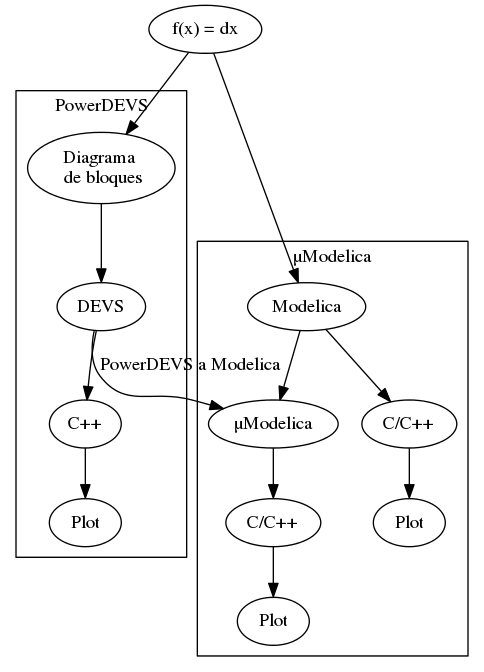
\includegraphics[width=0.75\linewidth]{esquema}
 \caption{Esquema de conversiones}
 \label{fig:esquema}
\end{figure}

En la figura \ref{fig:esquema}, se muestran los dos principales estrategias (PowerDEVS y Modelica) para realizar una simulación. En el caso de PowerDEVS, el primer paso es convertir el sistema en diagramas de bloques, luego en DEVS, en PowerDEVSe el cual puede automáticamente convertirlo en C++ y luego obtener los resultados ejecutando este modelo. Desde la perspectiva de Modelica (o $\mu$modelica, debemos pasar el sistema a modelica (o $\mu$Modelica) y luego el compilador se encargara de generar código (usualmente C o C++) capaz de correr la simulación y obtener resultados.
El actual trabajo esta representado por la flecha que sale de PowerDEVS hacia $\mu$modelica, permitiendo especificar la simulación en diagramas de bloques y ejecutar la simulación en el solver QSS, en el lenguaje $\mu$modelica.

\section{Organización del presente trabajo}

\section{Motivación y Objetivos}
PowerDEVS\cite{BK11} es una herramienta de simulación de sistemas híbridos, basado en el formalismo DEVS\cite{Zeigler:2000:TMS:580780}, con una interfaz gráfica orientada a bloques, donde los bloques pueden ser conectados entre si, modificado sus parámetros, además permite conectarse con el entorno Scilab para poder utilizar expresiones y herramientas de cálculo provistas por este entorno.

La resolución de ecuaciones diferenciales ordinarias, requiere el uso de métodos de integración numérica. Todos los algoritmos tradicionales de integración se basan en la discretización de la variable independiente (que generalmente representa el tiempo).

Las rutinas que implementan estos algoritmos, se denominan solvers y existen gran variedad de implementaciones de los mismos en diferentes lenguajes de programación. Los Métodos de Integración Numérica QSS (Quantized State System), a diferencia de los métodos de integración tradicionales, realizan la discretización sobre las variables de estado. En consecuencia, convierten los sistemas continuos en sistemas de eventos discretos, y tienen grandes ventajas para simular sistemas con discontinuidades.

Si bien PowerDEVS, implementa la totalidad de los algoritmos de QSS, resultan ineficientes, dado que malgastan gran parte de la carga computacional en la transmisión de eventos entre submodelos.

Para solventar este hecho se desarrollo una familia de QSS stand-solver, el cual requiere un modelo descripto en lenguaje C el cual contiene las ecuaciones diferenciales, las funciones de cruce de cero así como la información estructural requerida por los algoritmos QSS. Estos solvers obtienen una mejora de rendimiento de hasta un orden de magnitud comparado con otras implementaciones DEVS.

Sobre este se desarrollo una herramienta la cual genera a partir de un modelo $\mu$-Modedelica \cite{Ber12} (un subconjunto del lenguaje Modelica) el modelo requerido para el QSS solver.

Con el objetivo de utilizar los mejoras de velocidad y mantener un entorno amigable con el usuario, se creo una herramienta capas de convertir un modelo PowerDEVS en un modelo $\mu$modelica.


\section{Trabajo relacionado}
En \cite{Ber12} se describe una extensión del Compilador OpenModelica el cual traslada modelos regulares Modelica a $\mu$modelica. 
ModelicaDEVS \cite{Beltrame06quantisedstate} es una librería Dymola que permite describir simulaciones DEVS en el Modelica, más específicamente en el entorno Dymola.
M/CD++ \cite{conf/mascots/DAbreuW05} es una herramienta para convertir simulaciones en un subconjunto de Modelica, a simulaciones DEVS.
DESlib \cite{Sanz09paralleldevs} es una librería para la descripción de modelos Parallel DEVS en Modelica.


\section{Alcance}
DEVS\cite{Zeigler:2000:TMS:580780}, Discrete Event System Specification (Especificación de Sistemas de Eventos Discretos), es un formalismo modular y jerárquico para modelar y analizar sistemas que pueden ser de eventos de tiempo discreto mediante tablas de transición, y con estados continuos que pueden ser descriptos por ecuaciones diferenciales.
En el formalismo clásico DEVS, los modelos atómicos capturan el comportamiento del sistema, mientras los modelos Acoplados describen la estructura del mismo.
En particular los modelos atómicos en PowerDEVS son descriptos en clases C++, mientras que la estructura se encuentra definida en archivos pds y pdm.
Modelica es un lenguaje de modelado, orientado a objetos, declarativo, para el modelado orientado a componentes de sistemas complejos.
Para poder realizar nuestro objetivo es necesario primero contar con un modelo en modelica\cite{Fritzson02modelica--} para cada atómico PowerDEVS\cite{BK11} que deseemos convertir. 

De esto se desprenden las siguientes limitaciones importantes:
\begin{itemize}
	\item La semántica de los modelos convertidos depende de los modelos equivalentes a los DEVS atómicos 
	\item Solamente podemos convertir modelos cuyos componentes atómicos hayan sido convertidos a $\mu$modelica.
\end{itemize}


